\subsection{Level Terrain Specification}

\begin{figure}
\centering
  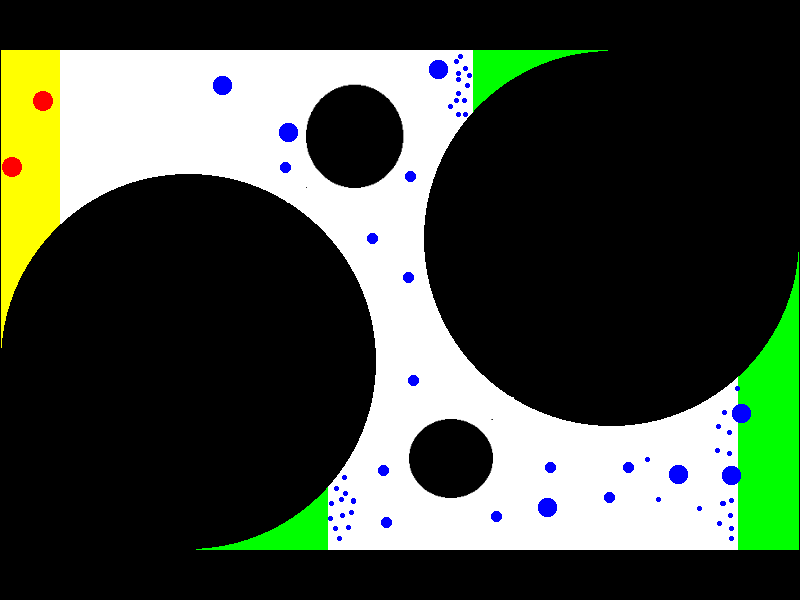
\includegraphics[scale=0.4]{img/ImageProcessing/LevelImages/img_0.png}
\caption{A typical player input for specifying the desired layout of the level\label{fig:LevelInput}}
\end{figure}

Figure \ref{fig:LevelInput} shows an example of a player's level specification.
\begin{itemize}
	\item Regions colored black represent land. This part of the domain is not a part of the solution field. The part of the black region that borders the white region is treated as a rigid boundary.
	\item White-colored regions represent the water body. This space is the actual solution domain of the fluid (i.e. the domain that the LBM solver works on).
	\item Green patches represent sources of momentum for the fluid.
	\item Yellow patches are sinks for the fluid. (See the section on LBM for the mathematical meaning of sources and sinks).
	\item Red spheres indicate the initial position of the players' boats.
	\item Blue spheres create obstacles as rigid bodies.
\end{itemize}
